\documentclass{article}
%% This is the preamble
    \usepackage[utf8]{inputenc}
    \usepackage[dvipsnames,svgnames,x11names,table]{xcolor}
    %% To customize page margins, use geometry
    \usepackage{geometry}
    \geometry{top=1.5in,left=1in, right=1in, bottom = 1.5in}
    %% physics and math packages
    \usepackage{amsmath,derivative,siunitx}
    %% some helpful packages to make internal links in your document
    \usepackage{hyperref}
    %% to include pictures and plots
    \usepackage{graphicx}
    % extra packages for Quantum
    \usepackage{braket}
    \renewcommand{\doteq}{\,\dot{=}\,}

\title{Homework 1}
\author{Adrian deCola}
\date{January 26, 2023}


%% Now we begin the formal document
\begin{document}

\maketitle


\section*{Problem 6.16}
    \verb+Problem+: Use $L=R\int_{\theta_1}^{\theta_2}{\sqrt{1 + \sin^2{\theta}(\phi'(\theta))^2}d\theta}$, the length of a path joining two points on a sphere of radius $R$ in spherical coordinates derived in Problem 6.1, to show that the shortest path, the geodesic, between two given points on a sphere is a great circle. 
    \hline
         \ \ \ 

    We want to minimize $L$:
    
    $$L=\int_{\theta_1}^{\theta_2}{f(\phi(\theta), \phi'(\theta), \theta)d\theta}$$
    
    where $f(\phi(\theta), \phi'(\theta), \theta)=R\sqrt{1 + \sin^2{\theta}(\phi'(\theta))^2}$. We can use the Euler-Lagrange equation to find stationary points for integrals of this form:
    
    $$\pdv{f}{\phi} - \odv{}{\theta}\left( \pdv{f}{\phi'}\right)=0$$

    Since $f=f(\phi'(\theta), \theta)$, 

    $$\pdv{f}{\phi}=0$$

    $$\odv{}{\theta}\left( \pdv{f}{\phi'} \right) = 0$$

    Using this, we find that $\pdv{f}{\phi'}=const.=k$.
    
    \begin{align*}
        k &= \pdv{f}{\phi'}\\
        k &= \pdv{}{\phi'}\left( R\sqrt{1 + \sin^2{\theta}(\phi'(\theta))^2}\right)\\
        k &=  R\left( \frac{1}{2} \right) \left( 1 + \sin^2{\theta}(\phi'(\theta))^2 \right)^{\frac{1}{2}} 2\sin^2{\theta}\phi'(\theta)\\
        k &= \frac{R\sin^2{\theta}\phi'(\theta)}{\sqrt{1 + \sin^2{\theta}(\phi'(\theta))^2}}\\
    \end{align*}

    Without loss of generality, we can make the z-axis go through Point 1. Using this point:

    $$\theta_1 = 0$$
    $$k = \frac{R\sin^2{0}*\phi'(0)}{\sqrt{1 + \sin^2{0}*(\phi'(0))^2}}=0$$

    We find that $k=0$. 

    \begin{align*}
        0 &= \frac{R\sin^2{\theta}\phi'(\theta)}{\sqrt{1 + \sin^2{\theta}(\phi'(\theta))^2}}\\
        0 &= R\sin^2{\theta}\phi'(\theta) \\
        0 &= \sin^2{\theta}\phi'(\theta)
    \end{align*}

    For this to be true for all $\theta$,

    $$\phi'(\theta)=0$$

    This means that $\phi(\theta)$ is constant, meaning the shortest path makes follows a great circle going through points 1 and 2 as shown in Figure 1 below. 
    \begin{figure}[!b]
        \centering
        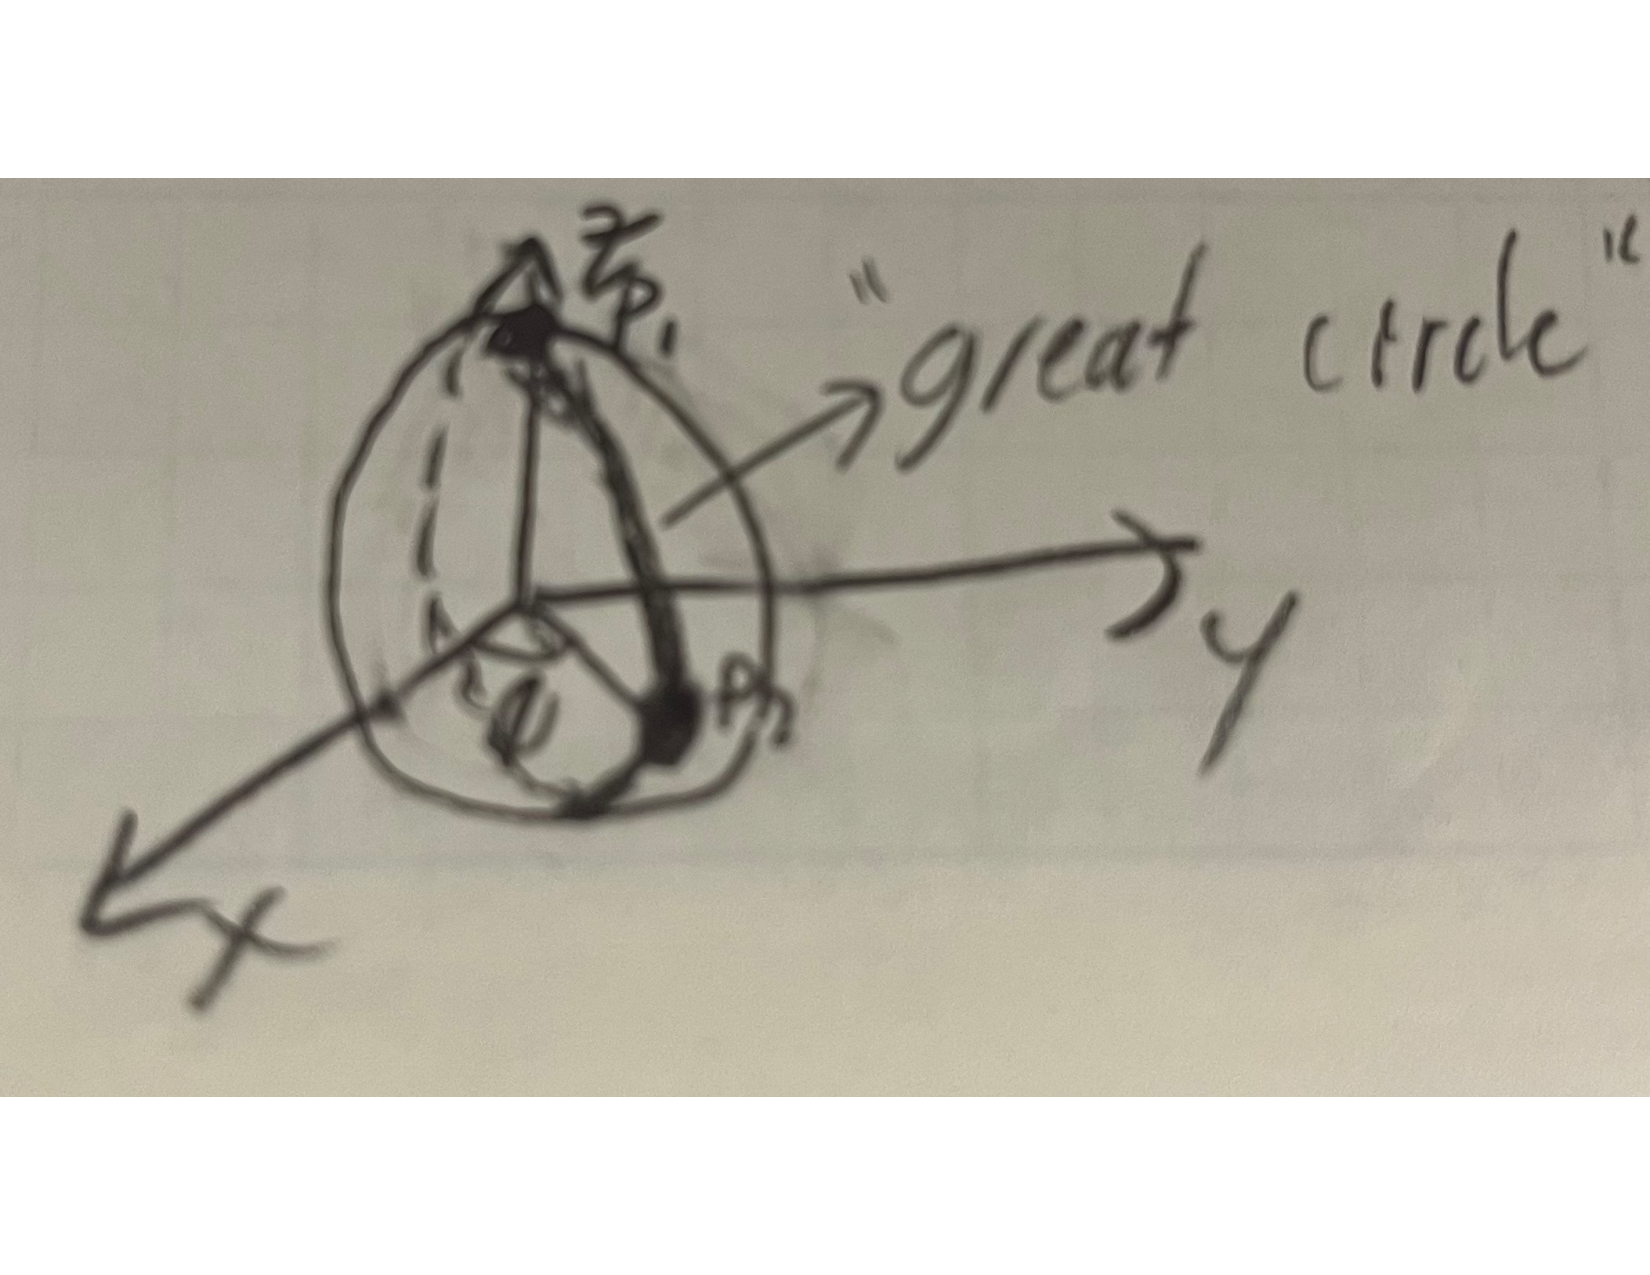
\includegraphics[width=0.5\textwidth]{HW_1_Fig_1.pdf}
        \caption{An illustration of the geodesic on a sphere where we have defined the z-axis to go through Point 1.}
    \end{figure}
    
  



\end{document}